% !TeX spellcheck = fa
\documentclass[a4paper,12pt]{report}

\usepackage{color}
\usepackage{float}
\usepackage{babel}
\usepackage{fourier}
\usepackage{amsmath}
%% \usepackage{dirtree} %to show tree view directories.
\usepackage{caption}
\usepackage{dirtree}
\usepackage{nomencl}
\usepackage{verbatim}
\usepackage{fancyhdr}
\usepackage{graphicx}
\usepackage{geometry}
\usepackage{outlines}
\usepackage{enumitem}
\usepackage{fancyvrb}
\usepackage{listings}
\usepackage{makecell}
\usepackage{tabularx} % for custom width table
\usepackage{subcaption}
\usepackage{datenumber}
\usepackage{indentfirst}
\usepackage{lstautogobble}
\usepackage[table]{xcolor}
\usepackage[utf8]{inputenc}
\usepackage[final]{pdfpages}
\usepackage[first=0, last=9]{lcg}
\usepackage[datesep=.,calc,showdow]{datetime2}
\usepackage{tikz}

%% \usepackage[perpage]{footmisc}
\usepackage[breakable]{tcolorbox}
\tcbuselibrary{breakable, skins}
\usepackage[Bjornstrup]{fncychap}
%Options: Sonny, Lenny, Glenn, Conny, Rejne, Bjarne, Bjornstrup
\usepackage[colorlinks,linkcolor=blue,citecolor=red,urlcolor=blue]{hyperref}

%% \usepackage[style=long,toc,xindy]{glossaries}
%% \usepackage[symbols,nogroupskip,sort=standard]{glossaries-extra}

\usepackage[fontsize={12,18}]{xepersian}

\DTMsetup{useregional}
% -------------- tcolorbox -------------
\tcbset{
	enhanced,
	colback=cyan!5!white,
	boxrule=0.1pt,
	colframe=cyan!75!black,
	fonttitle=\bfseries,
	width=0.9\linewidth
}

% ------------- font setup -------------
% ------------- xepersian --------------
%% \settextfont{Microsoft Sans Serif}
\settextfont{Yas}
\setlatintextfont{Times New Roman}
\setmathdigitfont{Yas}

\defpersianfont\XBT[Scale=1.1]{XB Titre}
\deflatinfont\FS[Scale=7]{Far.Symbol8}
\deflatinfont\TNR[Scale=1]{Times New Roman}

% --------------   xcolor  -------------
\definecolor{ao}{rgb}			{0.00, 0.50, 0.00}
\definecolor{codeGreen}{rgb}	{0.00, 0.50, 0.50}
\definecolor{lavendergray}{rgb}	{0.87, 0.86, 0.92}
\definecolor{mint}{rgb}			{0.24, 0.71, 0.54}
\definecolor{aliceblue}{rgb}	{0.94, 0.97, 1.00}
\definecolor{commentGreen}{rgb}	{0.13, 0.65, 0.47}
\definecolor{steelBlue}{rgb}	{0.00, 0.00, 0.50}
\definecolor{stringGreen}{rgb}	{0.00, 0.50, 0.00}
\definecolor{rowBlue}{rgb}		{0.48, 0.81, 0.87}

% ---------  page header setup ---------
% --------------  fancyhdr -------------
\pagestyle{fancy}

\cfoot{\thepage}
\rhead{\thepage }
\renewcommand{\headrulewidth}{0.4pt}

%% new commands.
\newcommand{\lrm}[1]{\textcolor{steelBlue}{\lr{\texttt{#1}}}}

%% tabular borders color
\arrayrulecolor{gray}

\renewcommand{\bibname}{مراجع}
% \newglossaryentry{dot-product}{name={dot product},description={aaa}}
% \makeglossaries
\makenomenclature
\renewcommand{\nomname}{فهرست علائم}
\nomenclature{$\bullet$}{bullet}

% ---------- arabic page numbering ------------
\makeatletter
\newcommand*{\@arabicalph}[1]{%
	\ifcase#1%
	\or
	آ%
	\or
	ب%
	\or
	ج%
	% ...
	\else
	\@ctrerr
	\fi
}
\newcommand*{\arabicalph}[1]{%
	\expandafter\@arabicalph\csname c@#1\endcsname
}
\makeatother


\begin{document}
	\lstset{
		frame		=	tb,
		basicstyle	=	\color{steelBlue}\linespread{0.8}\ttfamily,
		columns		=	fullflexible,
		keepspaces	=	false,
		tabsize		=	3,
		autogobble		,
		breaklines	=	true,
		breakatwhitespace=true,
		stringstyle	=	\color{stringGreen},
		commentstyle=	\color{gray},
		keywordstyle=	\color{purple},
		language	=	c++,
		aboveskip	=	3mm,
		belowskip	=	3mm,
		showstringspaces=false,
		columns		=	flexible,
		captionpos	=	b,
		numbers		=	left,
		numbersep	=	5pt,
		numberstyle	=	\color{gray}\linespread{0.8}\ttfamily,
		postbreak	=	\mbox{\textcolor{blue}{$\hookrightarrow$}\space}
	}

	\rand
	\title{
		{\vspace*{-5cm}
			\centering\quad\FS \arabic{rand}
		}\\[4cm]
		\XBT
		گیمبال
	}

	\date{
		\XBT
		\today
	}

	\pagenumbering{arabicalph}
	\maketitle
	\setcounter{page}{1}
	\tableofcontents
	%\printnomenclature
	\listoffigures
	%\listoftables

	\newpage
	\pagenumbering{arabic}

	\chapter{
	معرفی
	}\label{chap1}
	\rand
	\section{
	مقدمه
	}\label{sec1:chap1}

	دستگاه‌های حفط تعادل دوربین یا گیمبال
	\LTRfootnote{Gimbal}
	، به منظور حفظ تعادل دوربین در شرایط خاص استفاده می‌شوند.

	تعادل در 3 جهت
	\lr{x} و \lr{y}، \lr{z}
	کنترل می‌شود.

	در این دستگاه امکان مشخص کردن مسیر خودکار چرخش دوربین و یا تنظیم یک جهت ثابت نسبت به یک نقطه نیز فراهم است.

	\chapter{
		ساختار دستگاه
	}\label{chap2}
	این وسیله از دو بخش نرم‌افزار و سخت افزار و یک بدنه مکانیکی ایجاد شده است،‌که در ادامه به توضیحح هر یک پرداخته می‌شود.
	\section{ساختار فایل‌ها}\label{sec1:chap2}


	\begin{latin}
		\dirtree{%
			.1 .
			.1 \color{codeGreen} Document.
			.2 fonts.
			.2 resources.
			.1 \color{codeGreen} Extera.
			.2 3D Design Blender.
			.2 Circuit Design.
			.3 \color{orange}Main Board.
			.3 \color{orange}Main Board Altium.
			.4 Libraries.
			.4 \color{orange}PCB\_Project.
			.4 \color{orange}Power Supplay.
			.2 Data sheets.
			.2 Designs.
			.1 \color{codeGreen} Stabilizer Arduino.
			.2 stabilizer.
			.1 \color{codeGreen} Stabilizer ARM.
		}
	\pagebreak
	\paragraph{\rl{
			ادامه}}
		\dirtree{%
			.1 .
			.1 \color{codeGreen} Stabilizer Controller.
			.2 StabilizerController.
			.3 android.
			.3 controls.
			.4 NeumorphismStyle.
			.5 Dial.
			.3 resources.
			.4 application icon.
			.4 button svg image.
			.4 fonts.
			.3 model.
			.4 meshes.
			.3 views.
			.1 \color{codeGreen} UI Design.
			.2 outputs.
		}
	\end{latin}

	\section{
		بخش نرم‌افزاری
	}\label{sec2:chap2}
	بخش نرم‌افزاری این دستگاه به در فریم‌ورک
	\lr{Qt}
	و به صورت
	\lr{cross platform}
	توسعه داده شده است.
	بدین ترتیب امکان اجرای نرم‌افزار در سایر
	\lr{platform}
	ها ممکن است.

	فایل‌های برنامه کنترل کننده در زیر شاخه
	\lr{Stabilizer Controller/}
	قرار دارد.

	\subsection{
	\lr{veiw} ها}\label{subsec1:sec2:chap2}
		معرفی بخش‌های مختلف نرم‌افزار.

	برنامه کنترل‌کننده شامل چند بخش
	\lr{view}
	است، که به صورت
	\lr{stack}
	وار استفاده می‌شود.

	این بخش‌ها شامل:

	\begin{itemize}[nosep]
		\item
		پنل کنترل اصلی.
		\item
		پنل تنظیمات.
		\item
		پنل کنترل محدوده‌ای پیشرفته.
		\item
		پنل نمایش باتری.\\
		\danger
		(در حال حاظر پیاده سازی نشده)
		\item
		بخش
		\lr{joystick}
		مجازی.\\
		\danger
		(درحال حاظر پیاده سازی نشده)
	\end{itemize}

	\subsubsection{
	صفحه اصلی
	\lr{Control panel}}\label{subsec2:sec2:chap2}
	صفحه اصلی نرم‌افزار که در زیر قابل مشاهده است.
	این صفحه شامل بخش‌هایی است که در زیر به توضیح آن‌ها پرداخته می‌شود.
	\\


	\begin{figure}[!h]
		\centering

		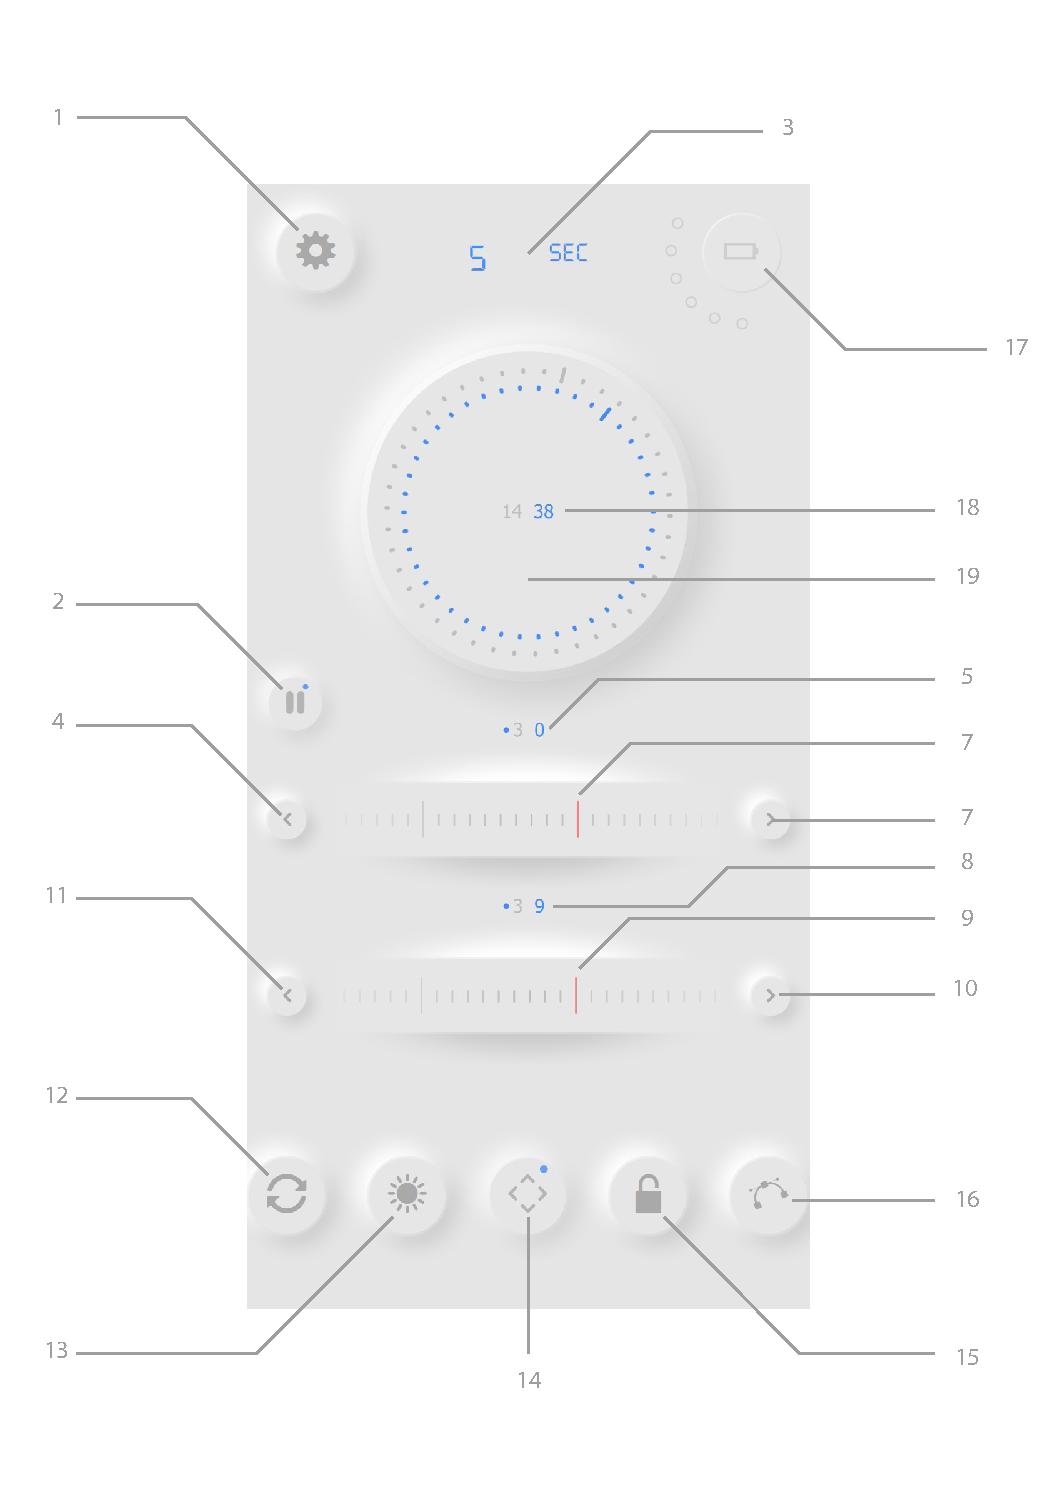
\includegraphics[width=0.6\textwidth]{resources/control-panel-labeled.pdf}
		\caption{
			صفحه کنترل‌کننده اصلی
		}
		\label{fig1:subsec2:sec2:chap2}
	\end{figure}

	\begin{enumerate}[nosep]
		\item
			باز کردن بخش تنظیمات نرم‌افزار.
		\item%2
			دکمه شروع و توقف
			\lr{timer}.

		\item
			ثانیه شمار، مقدار عدد وارد شده در این بخش ۴ رقم است و حداکثر مقدار
			$9999$
			ثانیه را می‌توان در این بخش قرار داد.

			درصورت قرار دادن مقدار صفر تایمر حرکت نخواهد کرد.
		\item%4
			دکمه مربوط به کاهش درجه محور
			\lr{x}.
			با فشار دادن این دکمه مقدار نشانگر یکی اضافه می‌شود و در صورت نگه‌داشتن، مقدار آن هر چند لحظه یکی اضافه می‌شود

		\item
		نشانگر درجه محور
		\lr{x}
		این نشانگر به صورت دو بخشی قرار دارد و بخش دوم به رنگ آبی و در سمت راست قرار دارد، که برای کاربرد مقدار دهی انتهای محدوده حرکت در حالت
		\lr{range mode}
		است.

		در صورت لمس و یا کلیک‌بر

		برای جابه‌جایی

		\item%6
			\lr{scroll}
			مربوط به کنترل محور
			\lr{x}.

			امکان حرکت به صورت
			\lr{flickable}
			را نیز دارد، مقادیر در صورت رسیدن به درجه پایانی از ابتدا شروع می‌شوند.
		\item

			دکمه مربوط به افزایش درجه محور
			\lr{x}.
			مابقی عملکرد مشابه مورد
			($ 4 $)
			است.
		\item%8
			نشانگر درجه محور
			\lr{y}
			عملکرد مشابه مورد
			$ (5) $
			است.
		\item
			کنترل‌کننده مربوط به درجه محور
			\lr{y}
			عملکرد مشابه مورد
			$ (6) $.
		\item%10
			افزایش درجه محور
			\lr{y}
			عملکرد مشابه مورد
			$ (4) $
			است.
		\item
			دکمه کاهش درجه محور
			\lr{y}
			عملکرد مشابه مورد
			$ (4) $
			است.
		\item%12
			دکمه مربوط به صفر کردن درجه تمامی محور‌ها.
		\item
			دکمه مربوط به جابه‌جایی بین حالت‌های شب و روز.
		\item%14
			دکمه مربوط به فعال‌سازی حالت محدوده‌ای، در این حالت می‌توان محدوده‌ای را برای حرکت دستگاه مشخص کرد، که طی زمانی که در بخش
			$ (3) $
			وارد می شود این حرکت انجام می‌پذیرد، بخش‌های دوگانه فقط مربوط به این حالت هستند و تنها در صورت لمس این دکمه فعال/غیرفعال می‌شوند.
		\item
			دکمه مربوط به قفل کردن موقعیت دستگاه در حالت فعلی.
		\item%16
			دکمه مربوط به بخش کنترل محدوده‌ای پیشرفته، که پنجره‌ای جدید برای کنترل بهتر دستگاه به صورت محدوده‌ای فراهم می‌کند. در این بخش که در ادامه توضیح داده خواهد شد، امکان قرار دهی موقعیت و زمان به صورت محدوده‌های خاص ممکن است.
		\item
			بخش مربوط نشانگر مربوط به نمایش باتری دستگاه، در صورت لمس دکمه به بخش نمایشگر مصرف باتری منتقل می‌شوید.

			\danger
			(این بخش در حال حاضر پیاده‌سازی نشده‌است)
		\item%18
			نشانگر درجه محور
			\lr{z}
			مشابه به بخش
			$ (5) $.
		\item
			کنترل کننده محور
			\lr{z}
			مشابه به مورد
			$ (6) $
			به صورت
			\lr{Dial}
			فراهم شده‌است، این بخش دارای دو
			\lr{Dial}
			تو در تو است، که برای مشخص کردن درجه شروع/حاضر دستگاه از نشانگر خراجی استفاده می شود.
			قسمت داخلی در صورت فعال شدن بخش
			$ (14) $
			نمایان می‌شود.
	\end{enumerate}

	\subsubsection{
		پنل کنترل پیشرفته محدوده‌ای
	}\label{subsec3:sec2:chap2}

	\begin{figure}[!h]
		\centering

		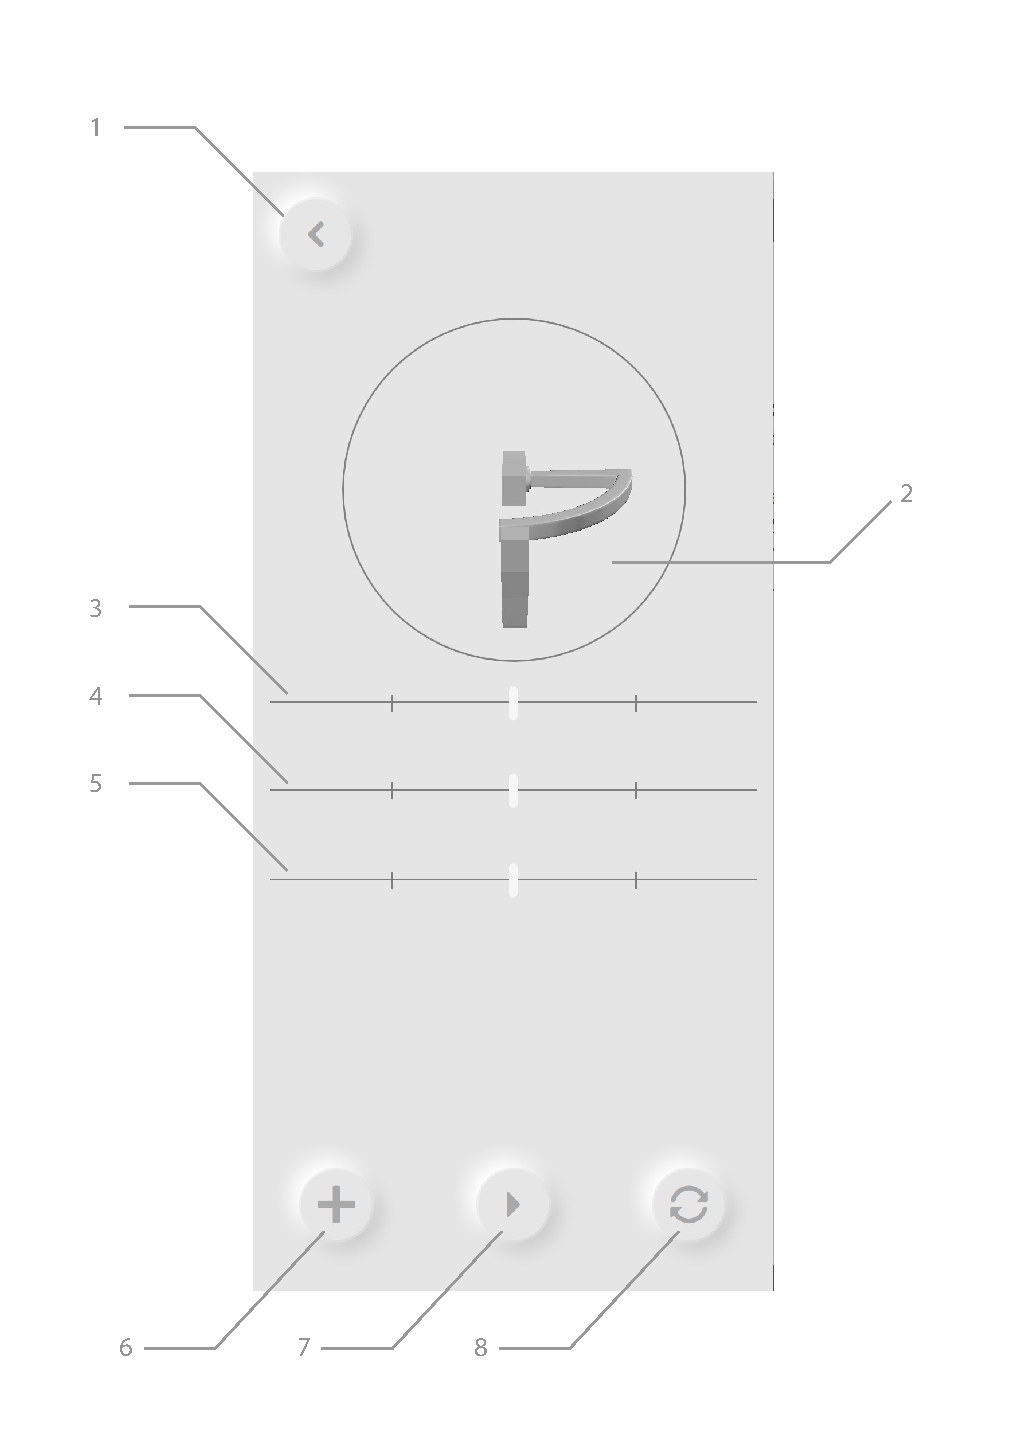
\includegraphics[width=0.6\textwidth]{resources/advanced-range-mode-labeled.pdf};
		\caption{
		صفحه حرکت در یک دامنه خاص و مدل سه بعدی
		}
		\label{fig2:subsec2:sec2:chap2}
	\end{figure}

	\begin{enumerate}[nosep]
		\item
			دکمه برگشت به پنل کنترل.
		\item
			نمایشگر
			$3D$
			از وضعیت فعلی دستگاه.
		\item
			کنترل محدوده‌ای مربوط به محور
			\lr{z}.

			\danger
			(در حال حاضر پیاده سازی کامل نشده‌است)
		\item
			کنترل محدوده‌ای مربوط به محور
			\lr{x}.

			\danger
			(در حال حاضر پیاده سازی کامل نشده‌است)
		\item
			کنترل محدوده‌ای مربوط به محور
			\lr{y}.

			\danger
			(در حال حاضر پیاده سازی کامل نشده‌است)
	\end{enumerate}

	\section{
	بخش سخت‌افزاری
	}\label{sec3:chap2}

	بخش سخت‌افزاری دد دو زیر بخش طراحی مدار و برنامه نویسی
	\lr{arduino}
	صورت گرفته است.

	و طراحی مدار نیز در برنامه‌های طراحی
	\lr{altium designer}
	و
	\lr{proteus}
	انجام شده، که نسخه‌های انتهایی در نرم‌افزار
	\lr{altium designer}
	طراحی شده است.

	مدار سخت‌افزاری از قطعات و ماژول‌هایی استفاده می‌کند که در زیر توضیح آنها آمده است.

	\paragraph{
	لیست ماژول‌ها و قطعات مورد استفاده}
	\begin{enumerate}[nosep]
		\item
			برای حرکت حول سه محور مختصاتی از
			$3$
			موتور
			\lr{servo}
			استفاده شده است، این موتور‌ها در حال حاضر با حداکثر
			\lr{$6$ volt}
			توانایی حرکت دارند، همچنین زاویه چرخش این موتور‌ها محدود به
			$180^{\circ}$
			درجه است، تحمل وزن در این موتور‌ها به حداکثر
			$ 6.5 $
			کیلوگرم در حالت
			\lr{stall}
			میرسد.

			این موتور‌ها در نسخه‌های بعدی با موتور‌های
			\lr{gearbox}
			دار و قابلیت چرخش
			$360^{\circ}$
			درجه جایگزین خواهند شد.
		\item
			حسگر جهت‌یاب به منظور تشخیص تغییر درجه در محور
			\lr{z}
			استفاده می‌شود، این ماژول با پروتکل
			\lr{I2C}
			با آردیونو ارتباط برقرار می‌کند.
		\item
			حسگر شتاب و زاویه سنج، از این حسگر به منظور سنجش درجه‌ و زاویه چرخش نسبت به محور‌های
			\lr{x}
			و
			\lr{y}
			استفاده می‌شود.

			\danger
			در حال حاضر برای تشخیص درجه چرخش، از محاسبه مقدار شتاب در جهت‌های
			\lr{x}، \lr{y} و  \lr{z}
			استفاده می‌شود.
		\item
			ماژول
			\lr{bluetooth}
			که از این ماژول برای ارسال اطلاعات بین دستگاه و نرم‌افزار استفاده می‌شود.
		\item
			چهار باتری
			\lr{2200 mA}
			 و
			\lr{3.3 Volt}
			که به صورت سری در دستگاه جایگذاری شده‌اند.
			   ‍
		\item
		مابقی قطعات شامل
		\lr{joystick}، \lr{rgb} \lr{led}، \lr{regulator}
		و
		$\dots$
		 است، که در برد استفاده شده و نیاز به توضیح ندارد.
	\end{enumerate}
	\subsection{
	برنامه‌نویسی
	\lr{arduino}}\label{subsec1:sec3:chap2}
	\subsubsection{
	مقدمه}
	\lr{arduino}\label{subsubsec1:subsec1:sec3:chap2}
	یک کمپانی سخت‌افزاری و نرم‌افزاری است که کیت‌های برد
	\lr{micro controller}
	را به صورت متن باز توسعه می‌دهد.

	این کیت سخت‌افزاری به منظور سهولت در ساخت مدل آزمایشی استفاده می‌شود.

	در این مدل از
	\lr{arduino nano}
	استفاده شده است که از
	\lr{micro controller}
	نوع
	\lr{ATMEGA32}
	استفاده می‌کند.

	\subsubsection{
	برنامه‌نویسی سخت‌افزار
	}\label{subsubsec2:subsec1:sec3:chap2}
	ساختار فایل‌های برنامه نوشته شده در
	\lr{arduino}
	به صورت زیر است.

	که شامل دستورات عملکرد

	که این کدها در هر دو سمت کنترل کننده و آردوینو برای ارسال دستورات از تفلن همراه به دستگاه مورد استفاده قرار می‌گیرد.

	همچنین کتابخانه مربوط به حالات
	\lr{LED}
	های نمایشگر موجود است که حالات آن‌ها را توصیف می‌کند.

	و در انتها  کد اصلی برنامه که شامل خواند درجات از حسگر‌ها و تنظیم زاویه موتورها است.
	\begin{latin}
		\dirtree{%
			.1 .
			.1 opCode.h.
			.1 stabilizer.cpp.
			.1 stabilizer.h.
			.1 stabilizer.ino.
			.1 statusled.cpp.
			.1 statusLED.h.
		}
	\end{latin}

	\subsection{
		طراحی برد
	}\label{subsec2:sec3:chap2}
		در این بخش با استفاده از نرم‌افزار قدرتمند طراحی برد
		\lr{altium designer}
		برد نهایی طراحی شده است.

		مجموعه برد نهایی در
		$ 3 $
		بخش
		\begin{itemize}[nosep]
			\item
				برد اصلی
			\item
				منبع برق، ‌که شامل ورودی برق است.
			\item
				کنترل‌کننده، که شامل
				\lr{joystick}
				و
				\lr{led}
				ها می‌باشد.

				\danger
				(در حال حاضر طراحی نشده)
		\end{itemize}

	\subsubsection{
	برد اصلی
	}\label{subsubsec1:subsec2:sec3:chap2}
		برد اصلی به منظور اتصال حسگر‌ها به آردوینو و حرکت موتور‌ها طراحی شده‌است.
		همچنین کنترل میزان شارژ شدن و قطع و وصل شدن باتری پس از شارژ توسط این برد انجام می‌گیرد.

		عکس‌های مربوط به لایه بالایی و لایه زیرین این برد در زیر آمده‌است.

		\begin{figure}[!h]
			\centering
			\begin{subfigure}{0.6\linewidth}
				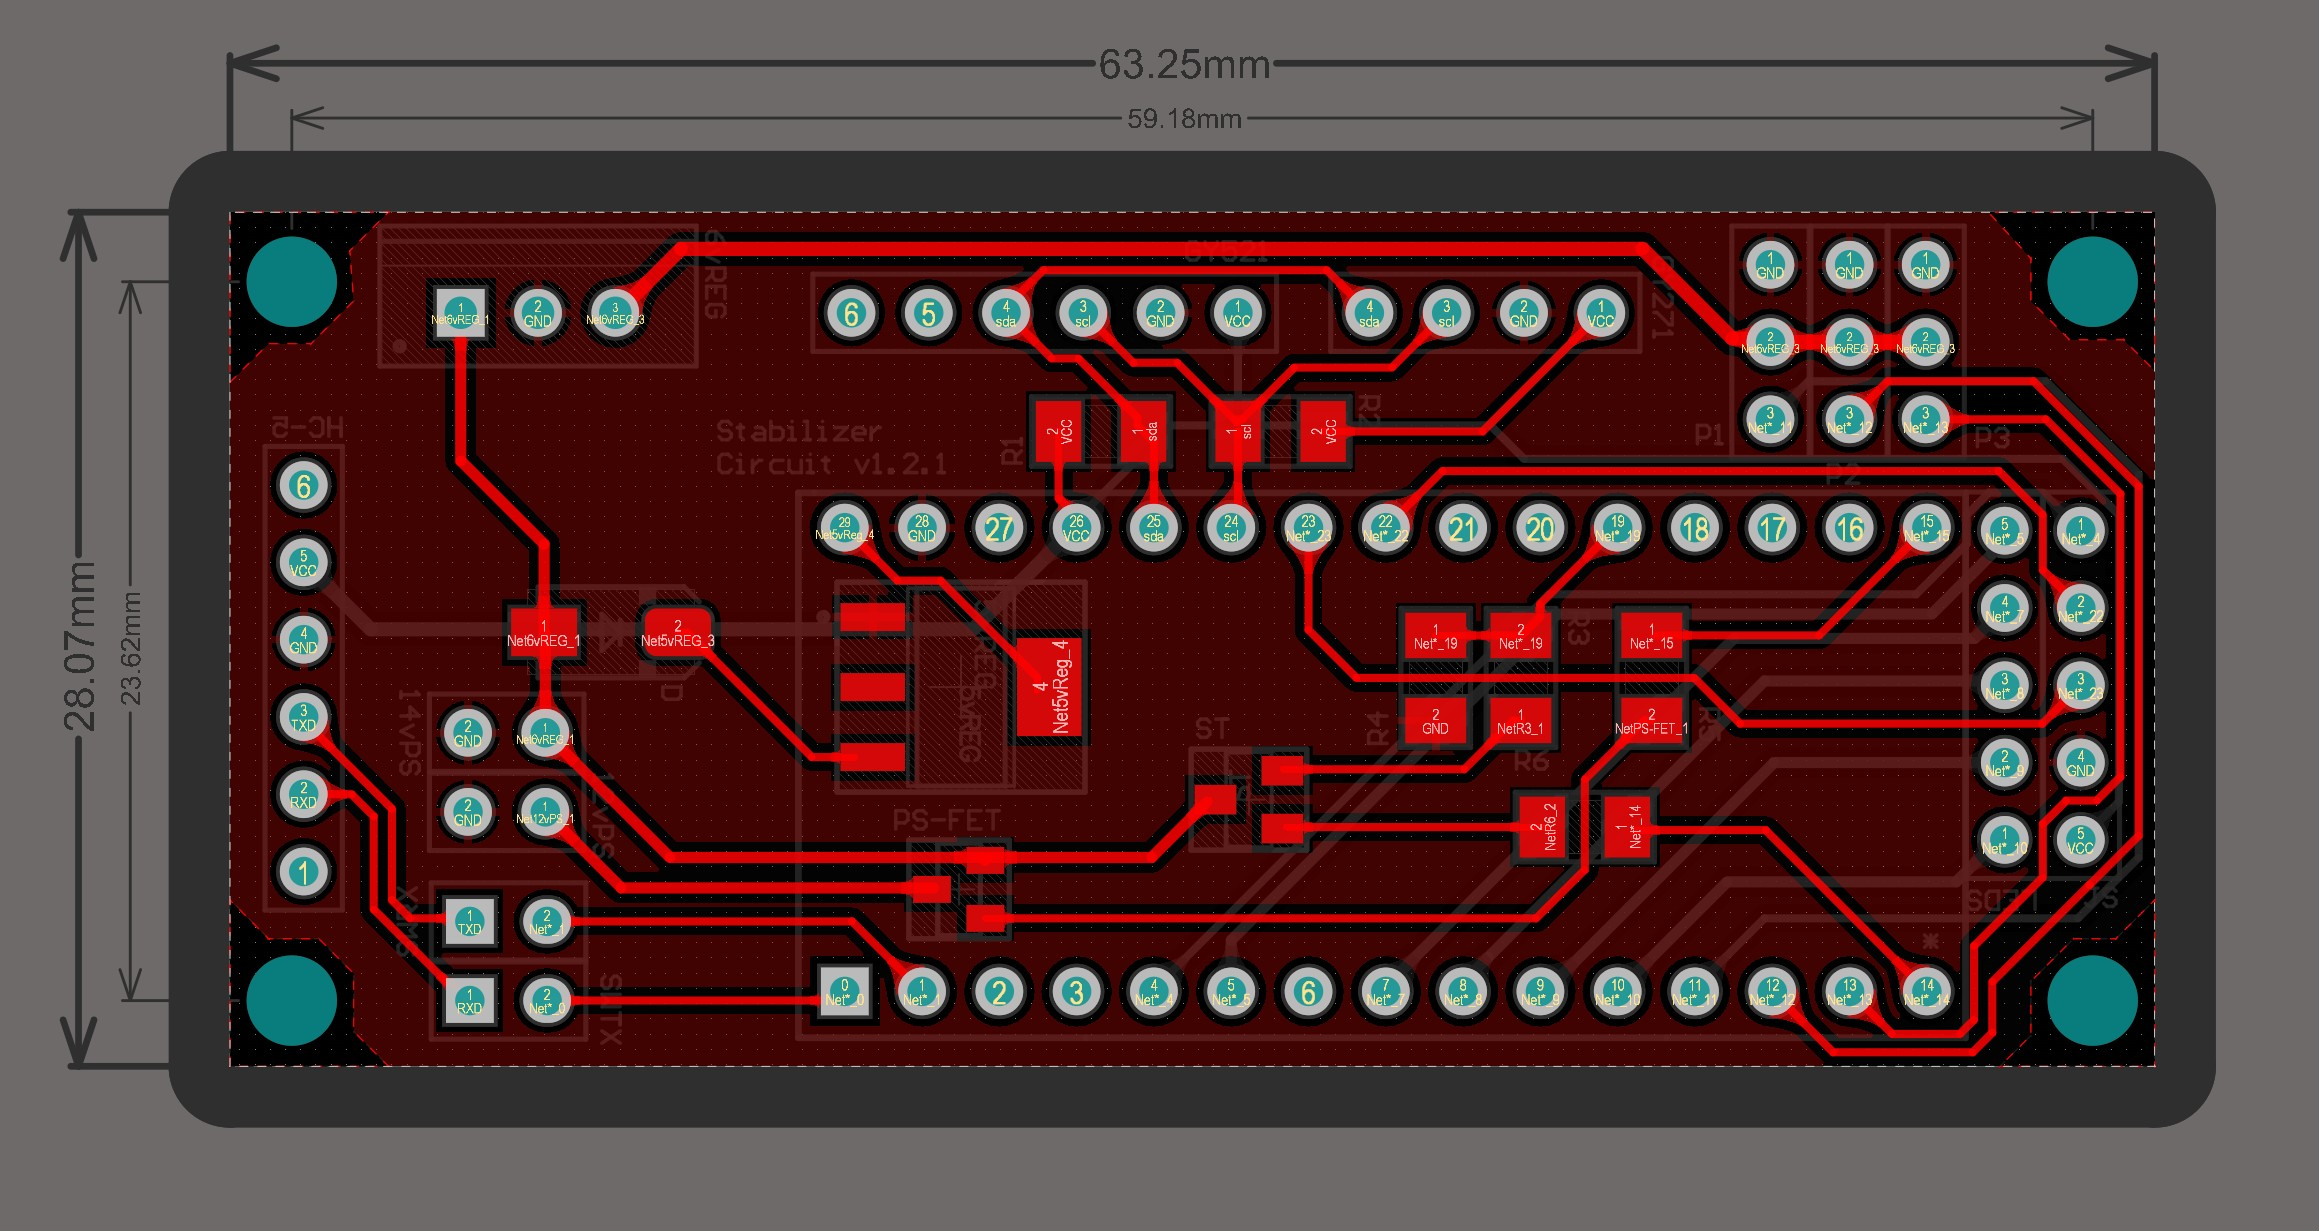
\includegraphics[width=0.9\linewidth]{resources/altium-main-board-top-layer.jpg}
				\caption{
				برد اصلی
				\lr{top layer}}
				\label{subfig1:fig1:subsubsec2:subsec2:sec3:chap2}
			\end{subfigure}\vspace*{5mm}
			\begin{subfigure}{0.6\linewidth}
				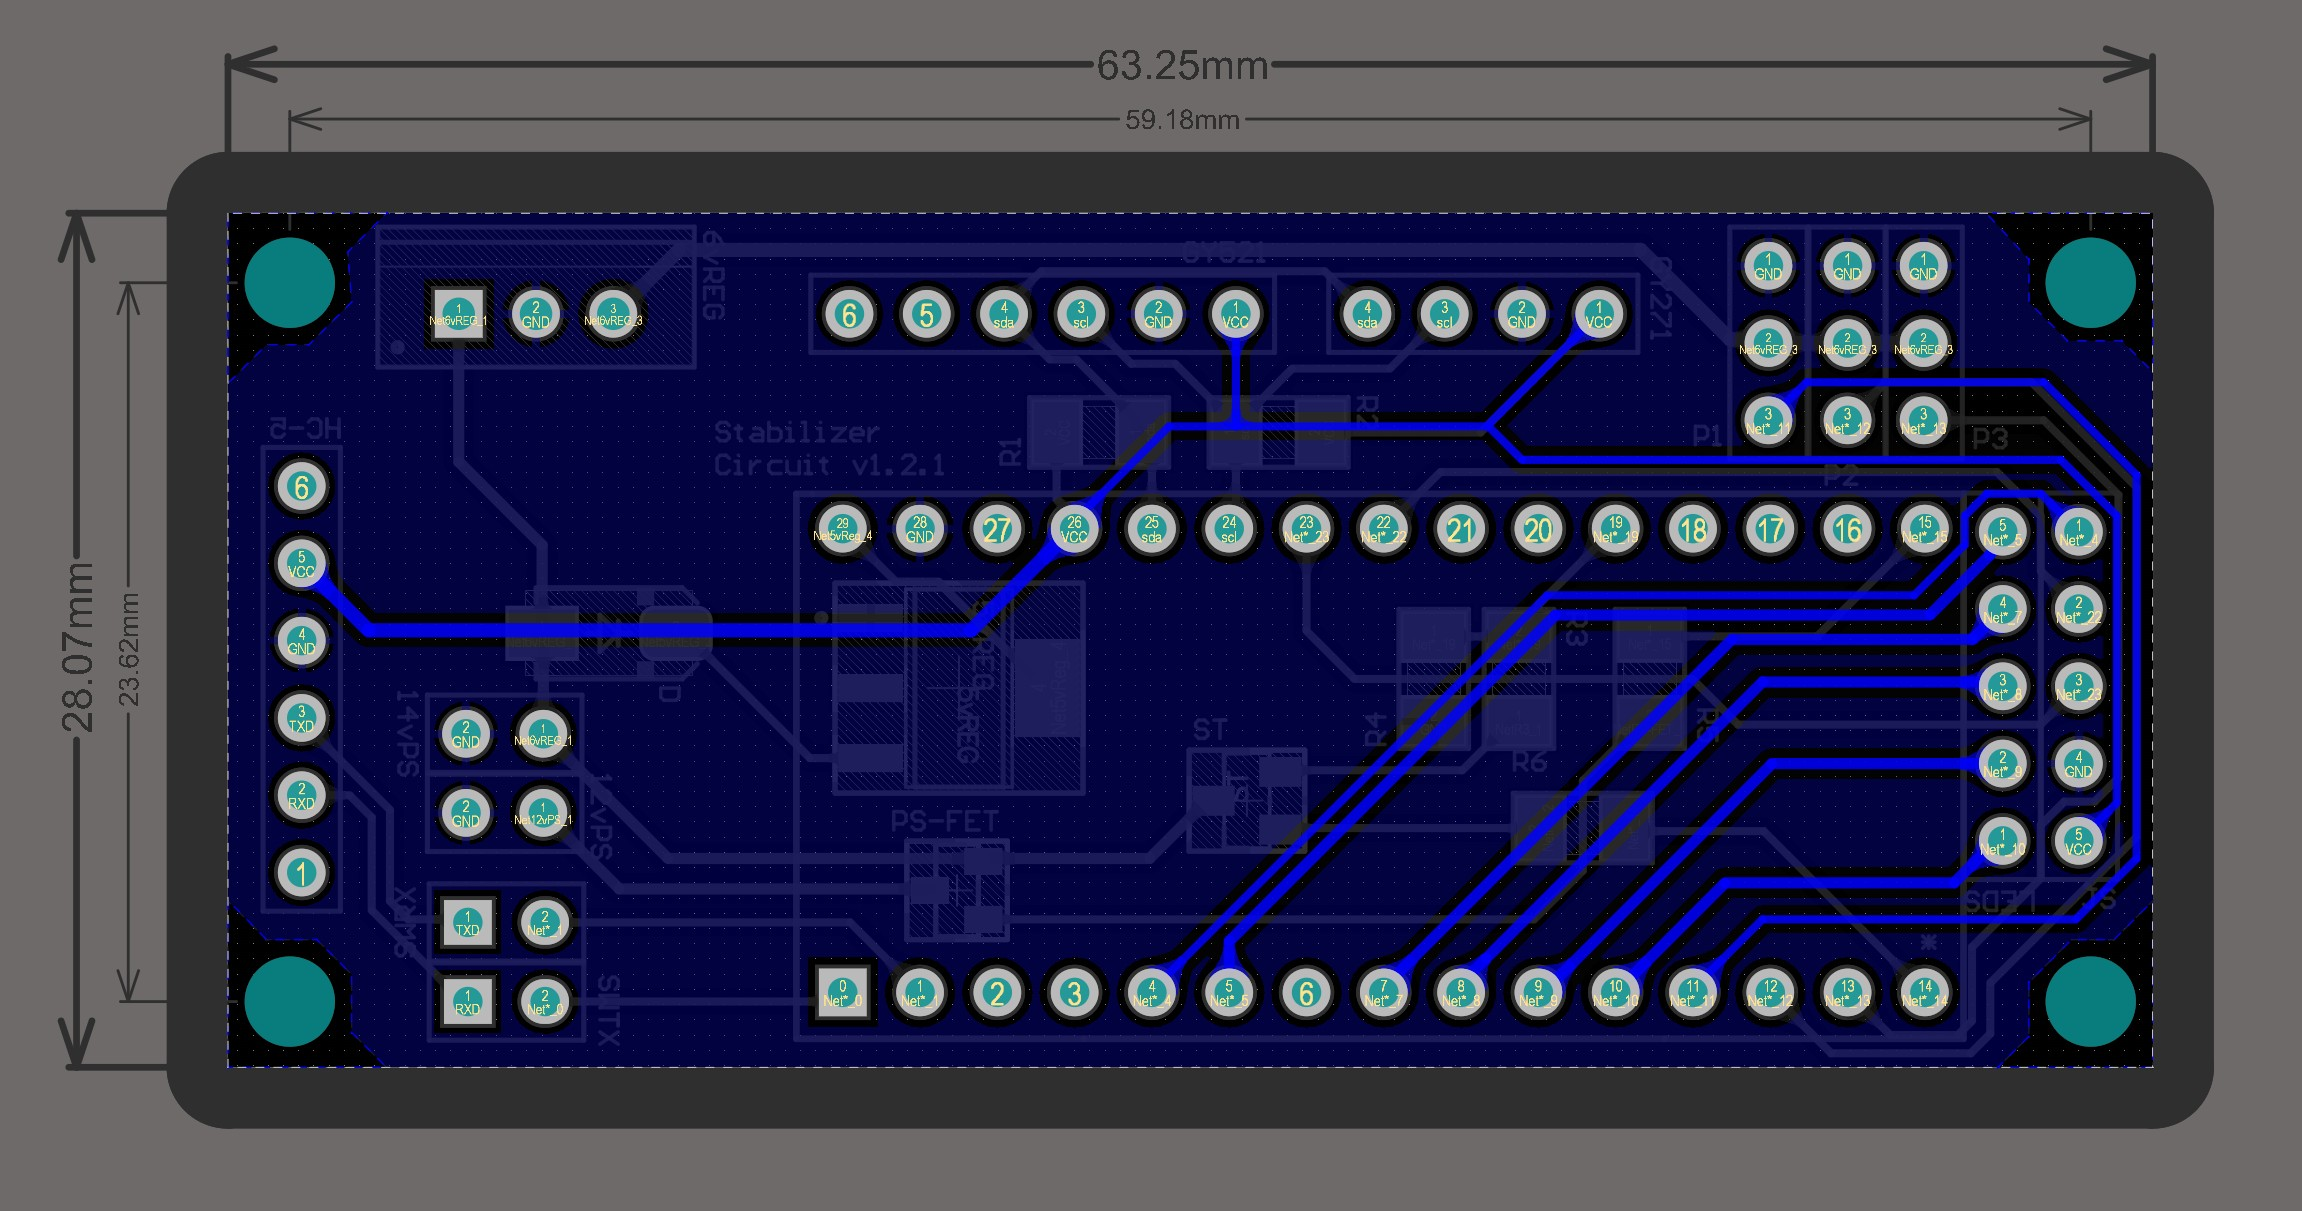
\includegraphics[width=0.9\linewidth]{resources/altium-main-board-bottom-layer.jpg}
				\caption{
				برد اصلی
				\lr{bottom layer}}
				\label{subfig2:fig1:subsubsec2:subsec2:sec3:chap2}
			\end{subfigure}
			\caption{
			برد اصلی}
			\label{fig1:subsubsec2:subsec2:sec3:chap2}
		\end{figure}

	\pagebreak
	\subsubsection{
		برد ورودی تغذیه
	}\label{subsubsec2:subsec2:sec3:chap2}
		این برد شامل یک قطعه
		\lr{micro USB}
		نری،‌است که به شارژر متصل می‌شود.

		ورودی منبع تغذیه باید یک برق مستقیم
		\lr{14 Volt}
		و با جریان تقریباً
		\lr{2 mA}
		باشد.

		مدار مذکور نیز در زیر آمده است.

		\begin{figure}[!h]
			\centering
			\begin{subfigure}{0.3\linewidth}
				\centering
				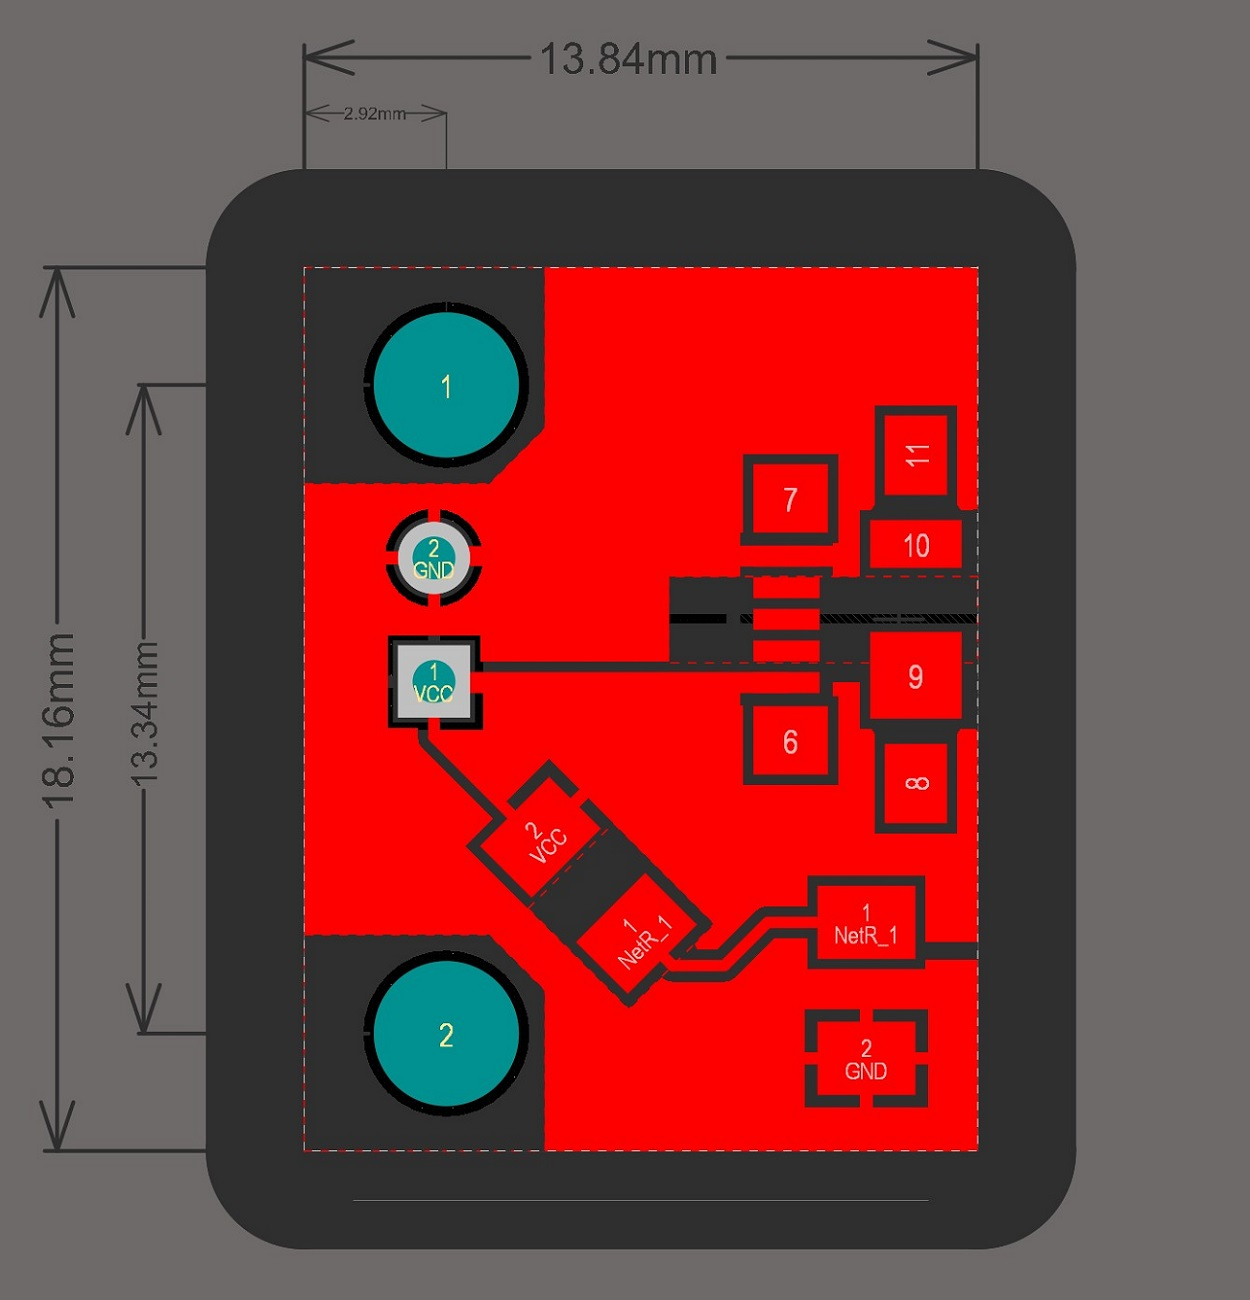
\includegraphics[width=0.7\linewidth]{resources/altium-power-supplay-top-layer.jpg}
				\caption{
				برد منبع تغذیه
				\lr{top layer}}
				\label{subfig1:fig1:subsubsec1:subsec2:sec3:chap2}
			\end{subfigure}
			\begin{subfigure}{0.3\linewidth}
				\centering
				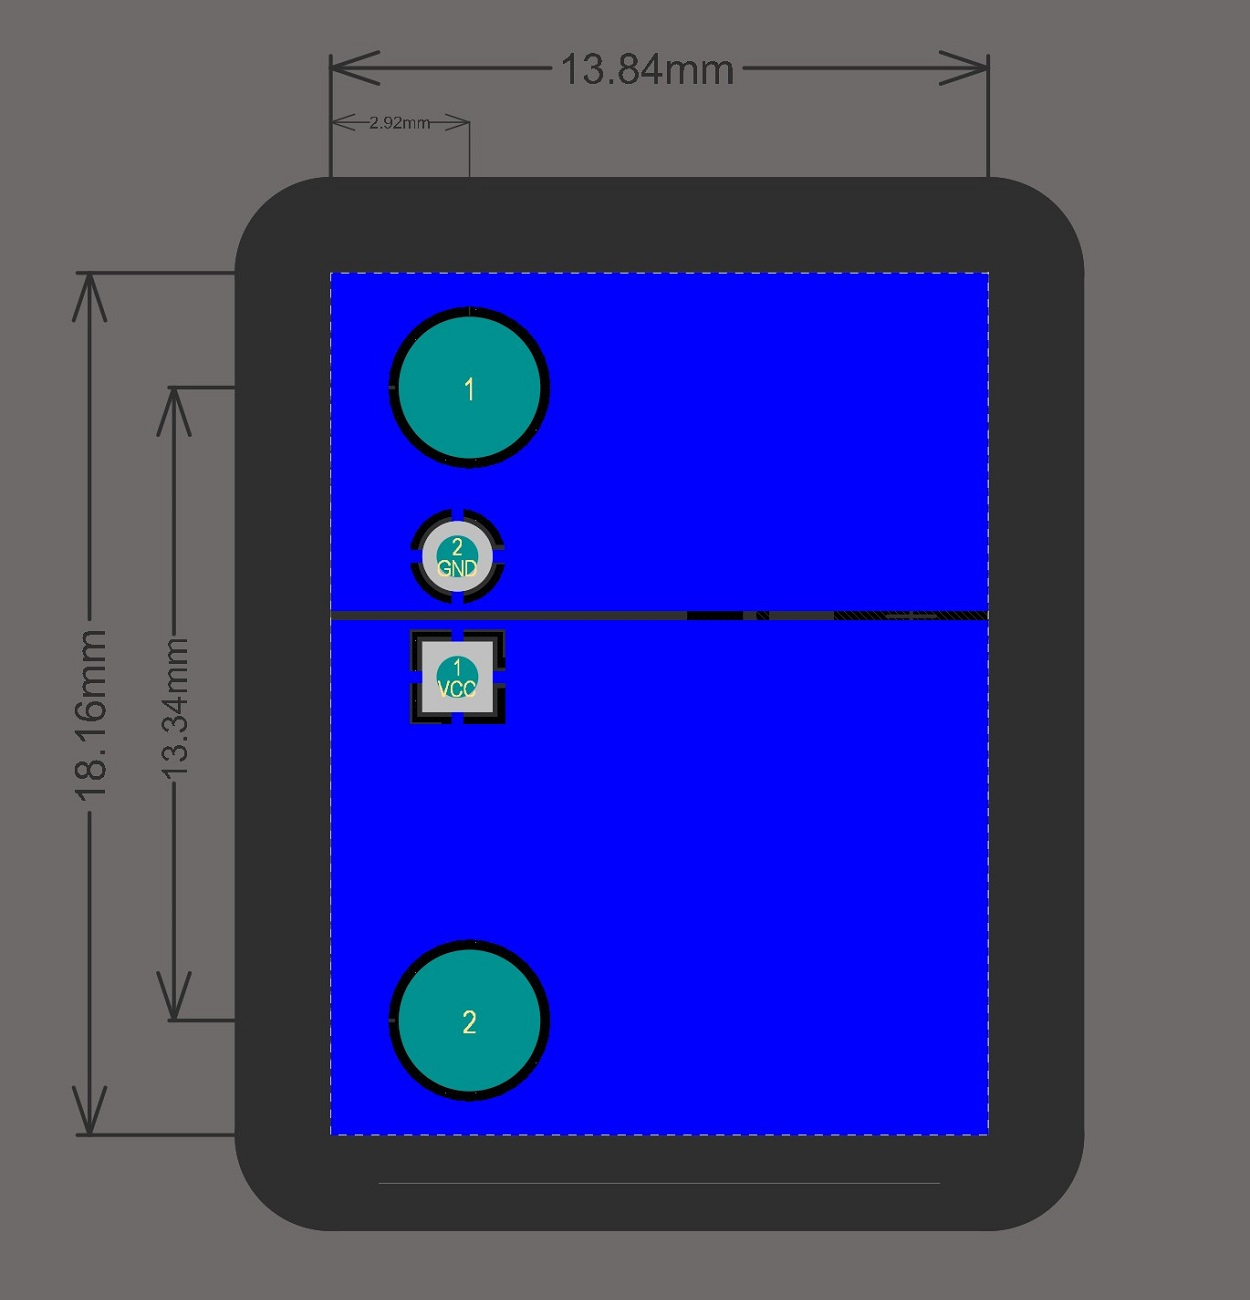
\includegraphics[width=0.7\linewidth]{resources/altium-power-supplay-bottom-layer.jpg}
				\caption{
				برد منبع تغذیه
				\lr{bottom layer}}
				\label{subfig2:fig1:subsubsec1:subsec2:sec3:chap2}
			\end{subfigure}
			\caption{
			برد منبع تغذیه}
			\label{fig1:subsubsec1:subsec2:sec3:chap2}
		\end{figure}

	\pagebreak
	\subsubsection{
		برد
		\lr{joystick}
	}\label{subsubsec3:subsec2:sec3:chap2}
	این برد مربوط به کلید‌ها و قطعات کنترلی دستگاه است.

	\danger
	(در حال حاضر این بخش در حال پروسه طراحی قرار دارد).
%	\begin{center}
%		\begin{tikzpicture}
%			\node[anchor=south west,inner sep=0]  at (0,0) {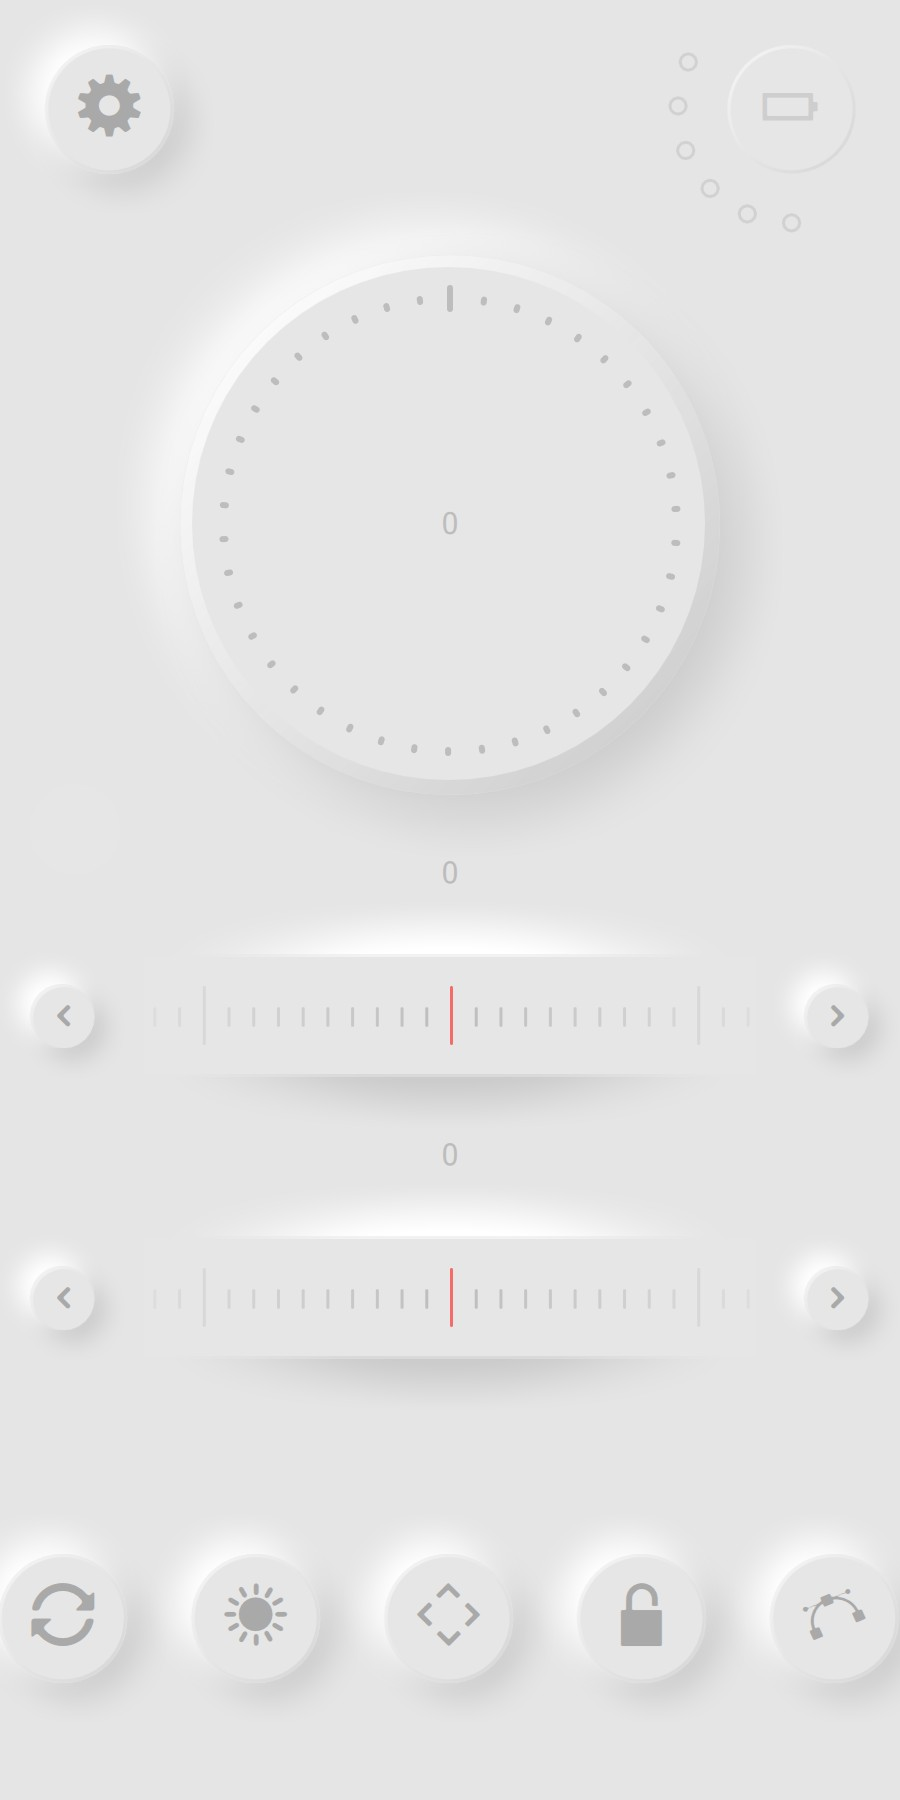
\includegraphics[width=0.3\textwidth]{resources/control-panel.jpg}};
%			\node[draw](x){};
%			\node[draw](y) at (2cm,0){};
%			\draw (x) to [bend left=10] (y);
%			\draw[red] (x.center) to [bend right=10] (y.center);
%		\end{tikzpicture}
%	\end{center}

%	\nocite{*}
%	\bibliographystyle{unsrt-fa}
%	\bibliography{refrence}
\end{document}